%!TEX root=../oi-magistr-si.tex
\section[NUR - Metody návrhu, uživatelské a konceptuální modely]{Metody návrhu, uživatelské a konceptuální modely}

\begin{figure}[h!]
\centering
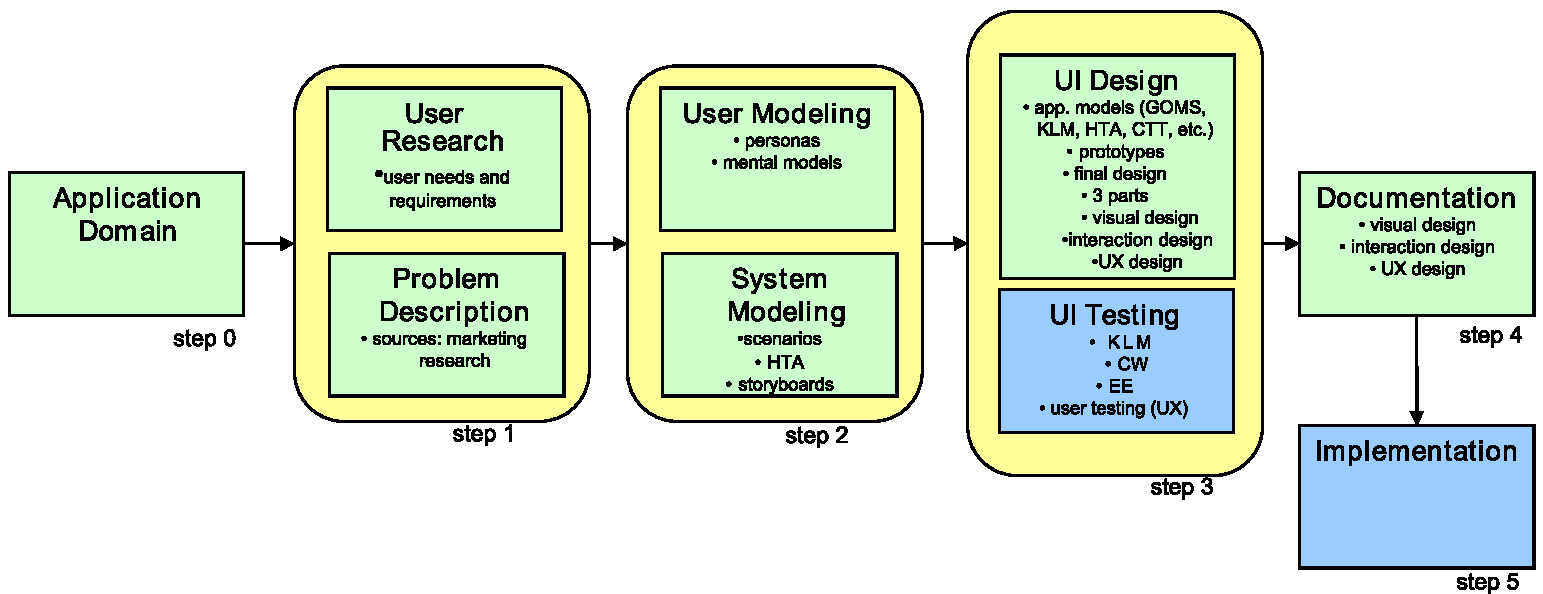
\includegraphics[width=125mm]{04/images/hci}
\end{figure}

\paragraph{Cyklus tvorby UI}
\begin{itemize}[itemsep=0px]
\item Návrh - porozumění uživateli (cílová skupina) a jeho potřebám
\begin{itemize}[itemsep=0px]
\item \textbf{analýza úlohy} - výkonnost software, hardware, uživatele při provádění úlohy, co uživatelé dělají, co k tomu potřebují za nástroje, co potřebují vědět, metoda: HTA
\item popis průběhu dialogu, slouží k následující implementaci UI
\end{itemize}
\item Implementace - prototypování
\item Vyhodnocení - hodnocení prototypu ve spolupráci s uživateli (kvalitativní \&
kvantitativní)
\item další iterace...
\end{itemize}

\paragraph{Analýza}
\begin{itemize}[itemsep=0px]
\item specifikace aktivit, které systém bude dělat
\item specifikace uživatelů - ti, kteří aktivity budou dělat
\item volba formy řešení - forma UI, SW podporující UI, OS, systémové požadavky, HW
\end{itemize}

\paragraph{Uživatel}
\begin{itemize}[itemsep=0px]
\item Uživatelské požadavky - Obecné požadavky: fyzické, kognitivní, sociální. Mohou být také specifické požadavky, které se vztahují přímo k problémmu.
\item Modely uživatele - KLM (Keystroke-level model), persony
\end{itemize}

\paragraph{Principy použitelného návrhu (usable design)}
\begin{itemize}[itemsep=0px]
\item jednoduché a přirozené dialogy v jazyku uživatele
\item konzistentnost akcí, příkazu, layoutu, terminologie
\item minimalizovat paměťovou zátěž uživatele - rozpoznávání je snazší než
vzpomínání
\item zpětná vazba
\item kontrola vstupu
\item snadné vrácení akcí - podpoří chuť experimentovat
\item výrazně značená ukončení - uživatel se nesmí ocitnout v pasti
\item zkratky - rychlé provedení časté akce pro zkušené uživatele
\item robustní systém poskytující snadno ovladatelné prostředky k nápravě chyb
\item užitečná nápověda a dobrá dokumentace (hledána v kritických situacích)
\end{itemize}

\paragraph{Terminologie}
\begin{itemize}[itemsep=0px]
\item Goal - to čeho chceme dosáhnout
\item Task - posloupnost aktivit, která dá \textit{goal}
\item Action - krok nebo akce - část \textit{tasku}
\end{itemize}

\subsection{Specifikace požadavků}
\begin{itemize}[itemsep=0px]
\item HTA (Hierarchical task analysis) - dekompoziční strom, kde je \textit{goal} zakreslen do postupně se rozpadajících menších \textit{tasků}. (CTT\footnote{Concurrent Task Tree} - strom s operátory a symboly)
\item Storyboard - série snímků a skeč§ (\uv{komiks} popisující \textit{goal})
\item Scénáře - jednoduché výpravné příběhy průběhu úkoli \textit{\uv{Uživatel napíše všechny účastníky akce, poté systém zkontroluje zda je vše vyplněno v pořádku a vytvoří událost...}}.
\item Případy užití - popis interakce člověka se systémem.
\end{itemize}

\subsection{Uživatelský průzkum}
Získávání informací o budoucích uživatelech systému, jejich \textbf{potřeby, zvyky , zkušenosti a dovednosti}.

\begin{itemize}[itemsep=0px]
\item \textbf{kvalitativní} - menší vzorek lidí, více informací, rozhovor, etnografické (pozorování chování) pozorování
\item \textbf{kvantitativní} - více lidí, méně informací, průzkumy, testy, pozorování
\item kombinovaný
\end{itemize}

\paragraph{Persona}
Detailně popsaný hypotetický uživatel reprezentující nějakou uživatelskou skupinu. Je založen na nasbíraných informacích. Nevýhody mohou být: nekonzistentní uživatel, představování si sama sebe jako uživatele.

\paragraph{Metody sběru dat}
\begin{itemize}[itemsep=0px]
\item pozorování - introspekce (sebepozorování) - zahrnuje kognitivní průchod, extrospekce
\item rozhovor - strukturovaný vs. volný, být neutrální a zvědavý (30-90 min), přímé otázky, žádná anonimita, vliv tazatele
\item dotazování (průzkum) - jednoduché otázky, používat rozsahy, neopakovat otázky, lidé lžou (chtějí vše, levně a ihned)
\item experiment
\end{itemize}

\subsection{Modely pro návrh UI}
\textbf{Konceptuální} model (design model) znamená to, jak to je navrženo. \textbf{Uživatelský} model (user model) značí co uživatel očekává. Nesoulad modelů vede k pomalému provádění úloh, chybám a frustraci

\paragraph{Mentální model} Uživatelovo porozumění jak se objekty chovají a jak akce prováděné přes UI ovlivňují jejich chování získané na základě zkušeností. Očekávané struktury a chování (menu, ukládání souborů, zpětná vazba, interpretace akcí). Vědomé i podvědomé procesy, které obsahují aktivaci obrazů a analogií. Hluboké a mělké modely (řízení auta vs. fungování auta).

UI musí prezentovat model vizuálně, mapování reálných prvků na rozhraní. Dobrý konceptuální model zahrnuje:
\begin{itemize}[itemsep=0px]
\item dostupnost funkcí (affordances)
\item návaznost (kauzalita)
\item omezení (constraints)
\item mapování jednotlivých kroků na akce
\item vzory chování cílových uživatelů
\end{itemize}
